\documentclass[12pt]{article}
\usepackage{graphicx}
\usepackage{wrapfig}
\usepackage{subfigure}
\usepackage{multirow}
\usepackage{hyperref}
\usepackage{amsmath}
\usepackage{amssymb}
\usepackage{ngerman}
\usepackage[ansinew]{inputenc}
\usepackage[left=2cm,top=1cm]{geometry}

% vector graphics test
\usepackage{color}
\usepackage{transparent}
\graphicspath{{graphs/}}





\begin{document}
	\pagestyle{empty}
	\textasciitilde

\begin{titlepage}
	\centering
	\bigskip
	\huge{Astronomisches Praktikum: Die Hubble-Konstante}\\
	\bigskip
	\large{Versuch 3}\\
	\bigskip
	\large{Jan R\"{o}der \& Julia Lienert}
	\bigskip
	\tableofcontents
\end{titlepage}

\pagebreak

\section{Einleitung}

\section{Methoden zur Entfernungsbestimmung}
\subsection{Cepheidenmethode}
Cepheiden sind Sterne, die ihre Helligkeit periodisch �ndern. Durch Beobachtung der Periode kann �ber die Perioden-Leuchtkraft-Beziehung
\begin{equation}
	M = -2.81 \log\left(\frac{P}{\text{Tage}}\right) -1.43
\end{equation}
auf die absolute Helligkeit geschlossen werden. Zusammen mit der scheinbaren (beobachteten) Helligkeit l�sst sich der Abstand �ber das Entfernungsmodul berechnen.
\begin{equation} \label{eq:Entfernungsmodul}
	m - M = 5 \log\left(\frac{r}{10\,\text{pc}}\right)
\end{equation}
Diese Methode ist bis zu einigen Megaparsec anwendbar. Mit dem Hubble-Space-Telescope k�nnen sogar Sterne in bis zu $20 \,$Mpc Entfernung beobachtet und vermessen werden, was eine Beobachtung auch in benachbarten Galaxien m�glich macht.
 
\subsection{Parallaxenmethode}
Bei dieser Methode wird die scheinbare Bewegung naher Sterne vor einem Fixsternhintergrund weit entfernter Sterne gemessen. Sie kommt dadurch zustande, dass sich die Erde im Lauf eines Jahres um die Sonne bewegt. \\
Gemessen wird - wie in Abbildung \ref{fig:Parallaxe} zu sehen ist - der sogenannte Parallaxenwinkel. �ber einfache Geometrie kann dann der Abstand des Sterns berechnet werden. Dazu muss der Abstand von der Erde zur Sonne bekannt sein (verwendet wird hierf�r der mittlere Kreisbahnradius von $1 \,$AE).
\begin{figure}
	\centering
	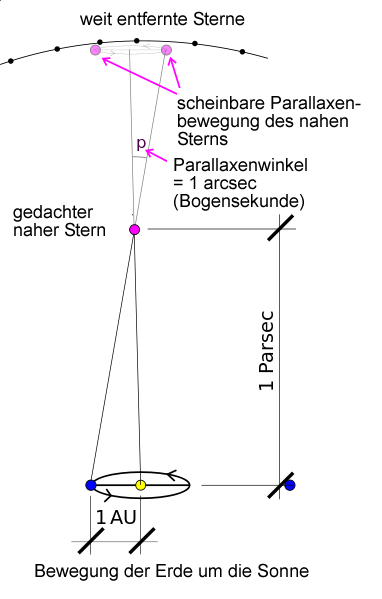
\includegraphics[width=0.3\textwidth]{Parallaxe.png}
	\caption{Skizze zur Erkl�rung der Parallaxe (entnommen aus [1])}
	\label{fig:Parallaxe}
\end{figure}
Entspricht der Parallaxenwinkel genau einer Bogensekunde, so wird die damit verkn�pfte Entfernung als $1 \,$pc bezeichnet. \\
Die Parallaxenmethode kann bis etwa $5000 \,$pc verwendet werden, wenn der Winkel mit dem Hubble-Space-Telescope gemessen wird.

\subsection{Supernova Typ 1a}
Da Supernovae vom Typ 1a immer gleiche Verl�ufe ihrer Lichtkurven haben, k�nnen sie - wie die Cepheiden - als Standardkerzen verwendet werden. Durch Aufnahme der Lichtkurve und Eichung auf eine Lichtkurve bekannten Abstands l�sst sich die Entfernung bestimmen. \\
Diese Methode hat eine Reichweite von �ber $1000 \,$Mpc, da Supernovae diesen Typs sehr leuchtkr�ftig sind.

\subsection{Kugelsternhaufen}
Alle Sterne in Kugelsternhaufen haben in etwa die gleiche Entfernung zu uns, deshalb ist auch die Differenz zwischen scheinbarer und absoluter Helligkeit (das Entfernungsmodul, siehe Gleichung \eqref{eq:Entfernungsmodul}) gleich. \\
Unter der Annahme, dass die Hauptreihensterne in Kugelsternhaufen im Hertzsprung-Russell-Diagramm die gleiche Kurve bilden wie die Sterne in Sonnenn�he, kann folgenderma�en der Abstand zu diesen Haufen bestimmt werden: Da die Kurven �bereinstimmen sollen, kann hieraus die absolute Helligkeit ermittelt werden. Durch Messen der scheinbaren Helligkeit kann aus dem Entfernungsmodul der Abstand des Haufens berechnet werden. \\ \\
Es gibt auch noch eine zweite Methode, mit der man mithilfe von Kugelsternhaufen Abst�nde bestimmen kann: Die Helligkeitsverteilung eines solchen Haufens folgt einer Gau�kurve, wobei die Position des Maximums bei konstanter absoluter Helligkeit liegt. Mithilfe der scheinbaren Helligkeit kann so wieder die Entfernung bestimmt werden. Hierf�r muss allerdings angenommen werden, dass sich der beobachtete Kugelsternhaufen genauso verh�lt wie diejenigen in der Milchstra�e. \\
Die Reichweite dieser Methode liegt bei $50 \,$Mpc.

\subsection{Tully-Fisher-Beziehung}
Die Tully-Fisher-Relation f�r Spiralgalaxien lautet:
\begin{equation}
	L \propto (v_{max})^{\beta}
\end{equation}
Die Leuchtkraft einer Spiralgalaxie ist somit proportional zur Potenz der maximalen Rotationsgeschwindigkeit dieser Galaxie. Die Potenz h�ngt vom betrachteten Spektralbereich ab. \\
Die Rotationsgeschwindigkeit erh�lt man aus der Verbreiterung der Spektrallinien: Diese sind verbreitert, da das Licht aus den sich auf uns zubewegenden Armen blauverschoben und das Licht aus den sich von uns wegbewegenden Armen rotverschoben ist. Je schneller sich die Galaxie dreht, umso st�rker wird dieser Effekt. \\
Andererseits h�ngt die Rotationsgeschwindigkeit einer Spiralgalaxie von deren Masse ab. Unter der Annahme, dass Galaxien mit gleicher Masse gleiche Leuchtkr�fte haben und die Leuchtkraft proportional zur Masse zunimmt, kann die absolute Helligkeit der Galaxie berechnet werden. Durch Messen der scheinbaren Helligkeit erh�lt man �ber das Entfernungsmodul wieder den Abstand der Galaxie. \\
Angewendet werden kann diese Methode f�r Entfernungen gr��er als $100 \,$Mpc.

\section{Messung der Hubble-Konstanten}
\subsection{Aufgabe 1}
Die Radialgeschwindigkeit ist diejenige Geschwindigkeitskomponente, die entlang der Sichtlinie des Beobachters zeigt. Gemessen werden kann sie durch Aufnahme eines Spektrums des auszumessenden Objekts. Vergleicht man die dort sichtbaren Spektrallinien mit bekannten, kann die Rotverschiebung ermittelt werden. Aus dieser erh�lt man direkt die Geschwindigkeit in radialer Richtung.

\subsection{Aufgabe 2}






\section{Quellen}
\begin{enumerate}
	\item https://de.wikipedia.org/wiki/Parallaxe
\end{enumerate}



\end{document}